\documentclass[11pt,letterpaper]{article}
\usepackage[lmargin=1in,rmargin=1in,tmargin=1in,bmargin=1in]{geometry}
\usepackage{../style/homework}
\usepackage{../style/commands}
\setbool{quotetype}{true} % True: Side; False: Under
\setbool{hideans}{false} % Student: True; Instructor: False

% -------------------
% Content
% -------------------
\begin{document}

\homework{11: Due 11/07}{What you learn from a life in science is the vastness of our igorance.}{David Eagleman}

% Problem 1
\problem{10} Plot the linear function $f(x)= \frac{2}{3}x - 4$ as accurately as possible.
	\[
	\fbox{
	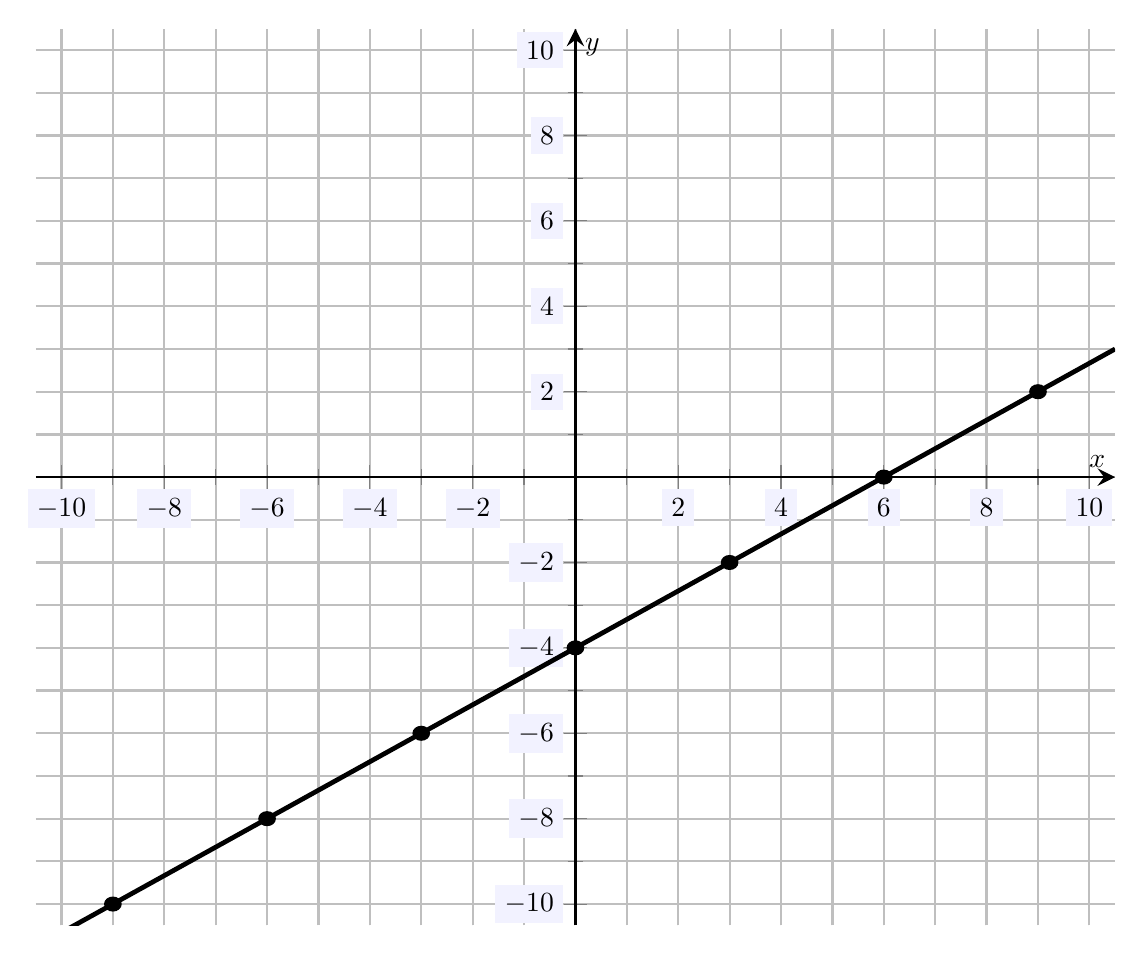
\begin{tikzpicture}[scale=2,every node/.style={scale=0.5}]
	\begin{axis}[
	grid=both,
	axis lines=middle,
	ticklabel style={fill=blue!5!white},
	xmin= -10.5, xmax=10.5,
	ymin= -10.5, ymax=10.5,
	xtick={-10,-8,-6,-4,-2,0,2,4,6,8,10},
	ytick={-10,-8,-6,-4,-2,0,2,4,6,8,10},
	minor tick = {-10,-9,...,10},
	xlabel=\(x\),ylabel=\(y\),
	]
	\addplot[domain=-10.5:10.5,black,line width=0.03cm] (x,2/3*x-4);
	\draw[fill=black] (-9,-10) circle (0.15);
	\draw[fill=black] (-6,-8) circle (0.15);
	\draw[fill=black] (-3,-6) circle (0.15);
	\draw[fill=black] (0,-4) circle (0.15);
	\draw[fill=black] (3,-2) circle (0.15);
	\draw[fill=black] (6,0) circle (0.15);
	\draw[fill=black] (9,2) circle (0.15);
	\end{axis}
	\end{tikzpicture}
	}
	\] \pspace

{\itshape We know that $f(x)= \frac{2}{3}x - 4$ is a linear function because it has the form $y= mx + b$ with $m= \frac{2}{3}$ and $b= -4$. The $y$-intercept is $-4$, i.e. $(0, -4)$. The slope is $\frac{2}{3}$, i.e. $\frac{\Delta y}{\Delta x}$. Then for each increase of 3 in $x$, there is an increase of 2 in $y$. Because $\frac{2}{3}= \frac{-2}{-3}$, this is equivalent to every 3 decrease in $x$ there is a decrease of 2 in $y$. Using these facts along with the $y$-intercept, we can plot the points on the graph above to create the line.}



\newpage



% Problem 2
\problem{10} Plot the linear function $f(x)= 7 - 2x$ as accurately as possible.
	\[
	\fbox{
	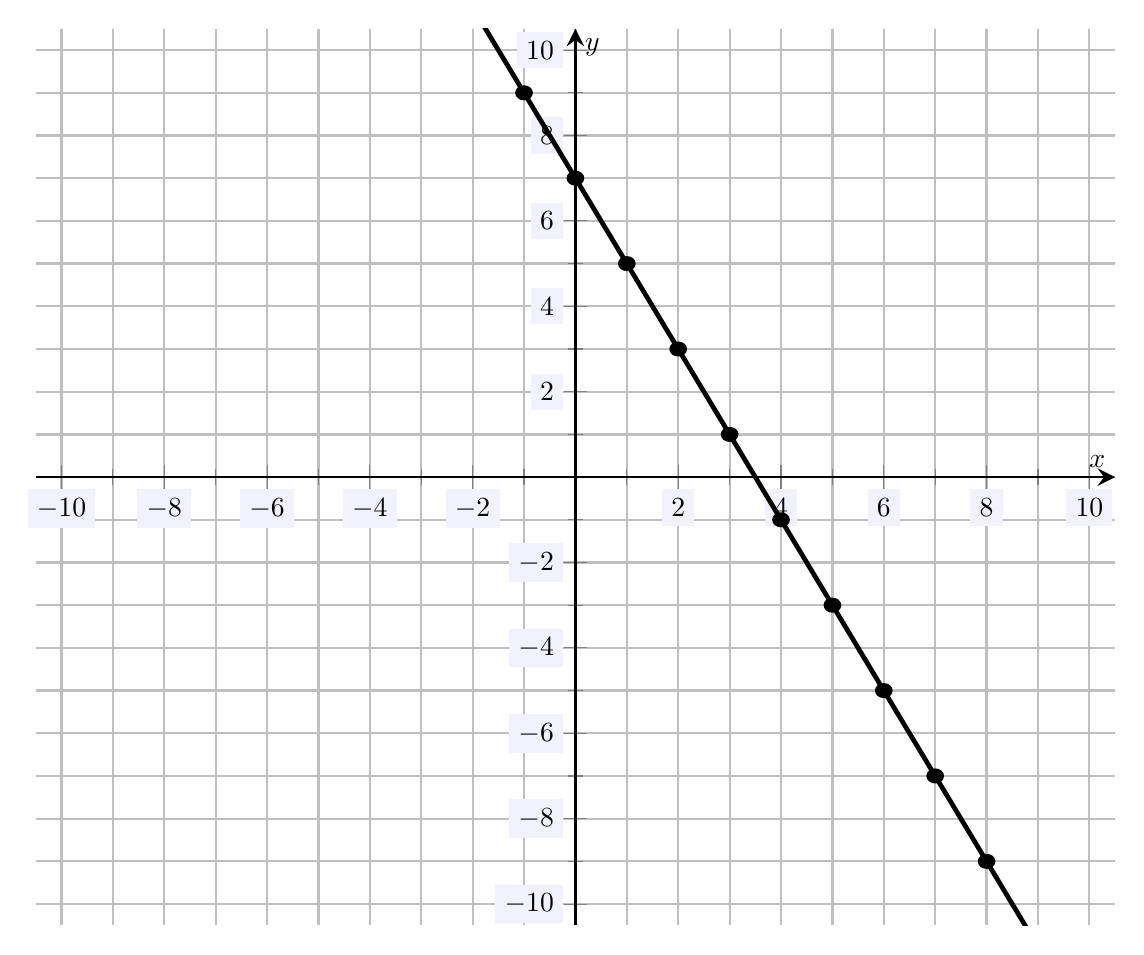
\begin{tikzpicture}[scale=2,every node/.style={scale=0.5}]
	\begin{axis}[
	grid=both,
	axis lines=middle,
	ticklabel style={fill=blue!5!white},
	xmin= -10.5, xmax=10.5,
	ymin= -10.5, ymax=10.5,
	xtick={-10,-8,-6,-4,-2,0,2,4,6,8,10},
	ytick={-10,-8,-6,-4,-2,0,2,4,6,8,10},
	minor tick = {-10,-9,...,10},
	xlabel=\(x\),ylabel=\(y\),
	]
	\addplot[domain=-10.5:10.5,black,line width=0.03cm] (x,7 - 2*x);
	\draw[fill=black] (-1,9) circle (0.15);
	\draw[fill=black] (0,7) circle (0.15);
	\draw[fill=black] (1,5) circle (0.15);
	\draw[fill=black] (2,3) circle (0.15);
	\draw[fill=black] (3,1) circle (0.15);
	\draw[fill=black] (4,-1) circle (0.15);
	\draw[fill=black] (5,-3) circle (0.15);
	\draw[fill=black] (6,-5) circle (0.15);
	\draw[fill=black] (7,-7) circle (0.15);
	\draw[fill=black] (8,-9) circle (0.15);
	\end{axis}
	\end{tikzpicture}
	}
	\] \pspace

{\itshape We know that $f(x)= 7 - 2x$ is a linear function because it has the form $y= mx + b$ with $m= -2$ and $b= 7$. The $y$-intercept is $7$, i.e. $(0, 7)$. The slope is $-2= \frac{-2}{1}$, i.e. $\frac{\Delta y}{\Delta x}$. Then for each increase of 1 in $x$, there is a decrease of 2 in $y$. Because $\frac{-2}{1}= \frac{2}{-1}$, this is equivalent to every 1 decrease in $x$ there is an increase of 2 in $y$. Using these facts along with the $y$-intercept, we can plot the points on the graph above to create the line.}


\end{document}